% Thesis chapter: introduction.
% Standalone chapter file; \input or \include from the thesis root.

\chapter{Introduction}
\label{ch:intro}

\section{Motivation}

The Canadian forestry sector is a cornerstone of the national economy, yet its
adoption of automation has lagged well behind comparable industries, a gap made
pressing by persistent skilled-labor shortages and by the safety demands of
operating heavy machinery around unstable loads~\cite{huq2007skills,
lindroos2017forestry}. Mill yards concentrate one of the sector's most
repetitive machine tasks: wood arrives in dense piles of logs that must be
grasped, transported, and deposited by grapple-equipped log loaders, cycle
after cycle, throughout a shift (Figure~\ref{fig:intro_mill}). Expert operators
perform this task with remarkable skill, judging where to sink the grapple in a
pile they can only partially see, capturing many logs at once without
destabilizing the remainder, and adapting continuously as each grasp reshapes
the pile. The work is also fatiguing, repetitive, and costly, which makes it a
natural target for autonomy~\cite{oliveira2021advances}.

\begin{figure}[t]
\centering
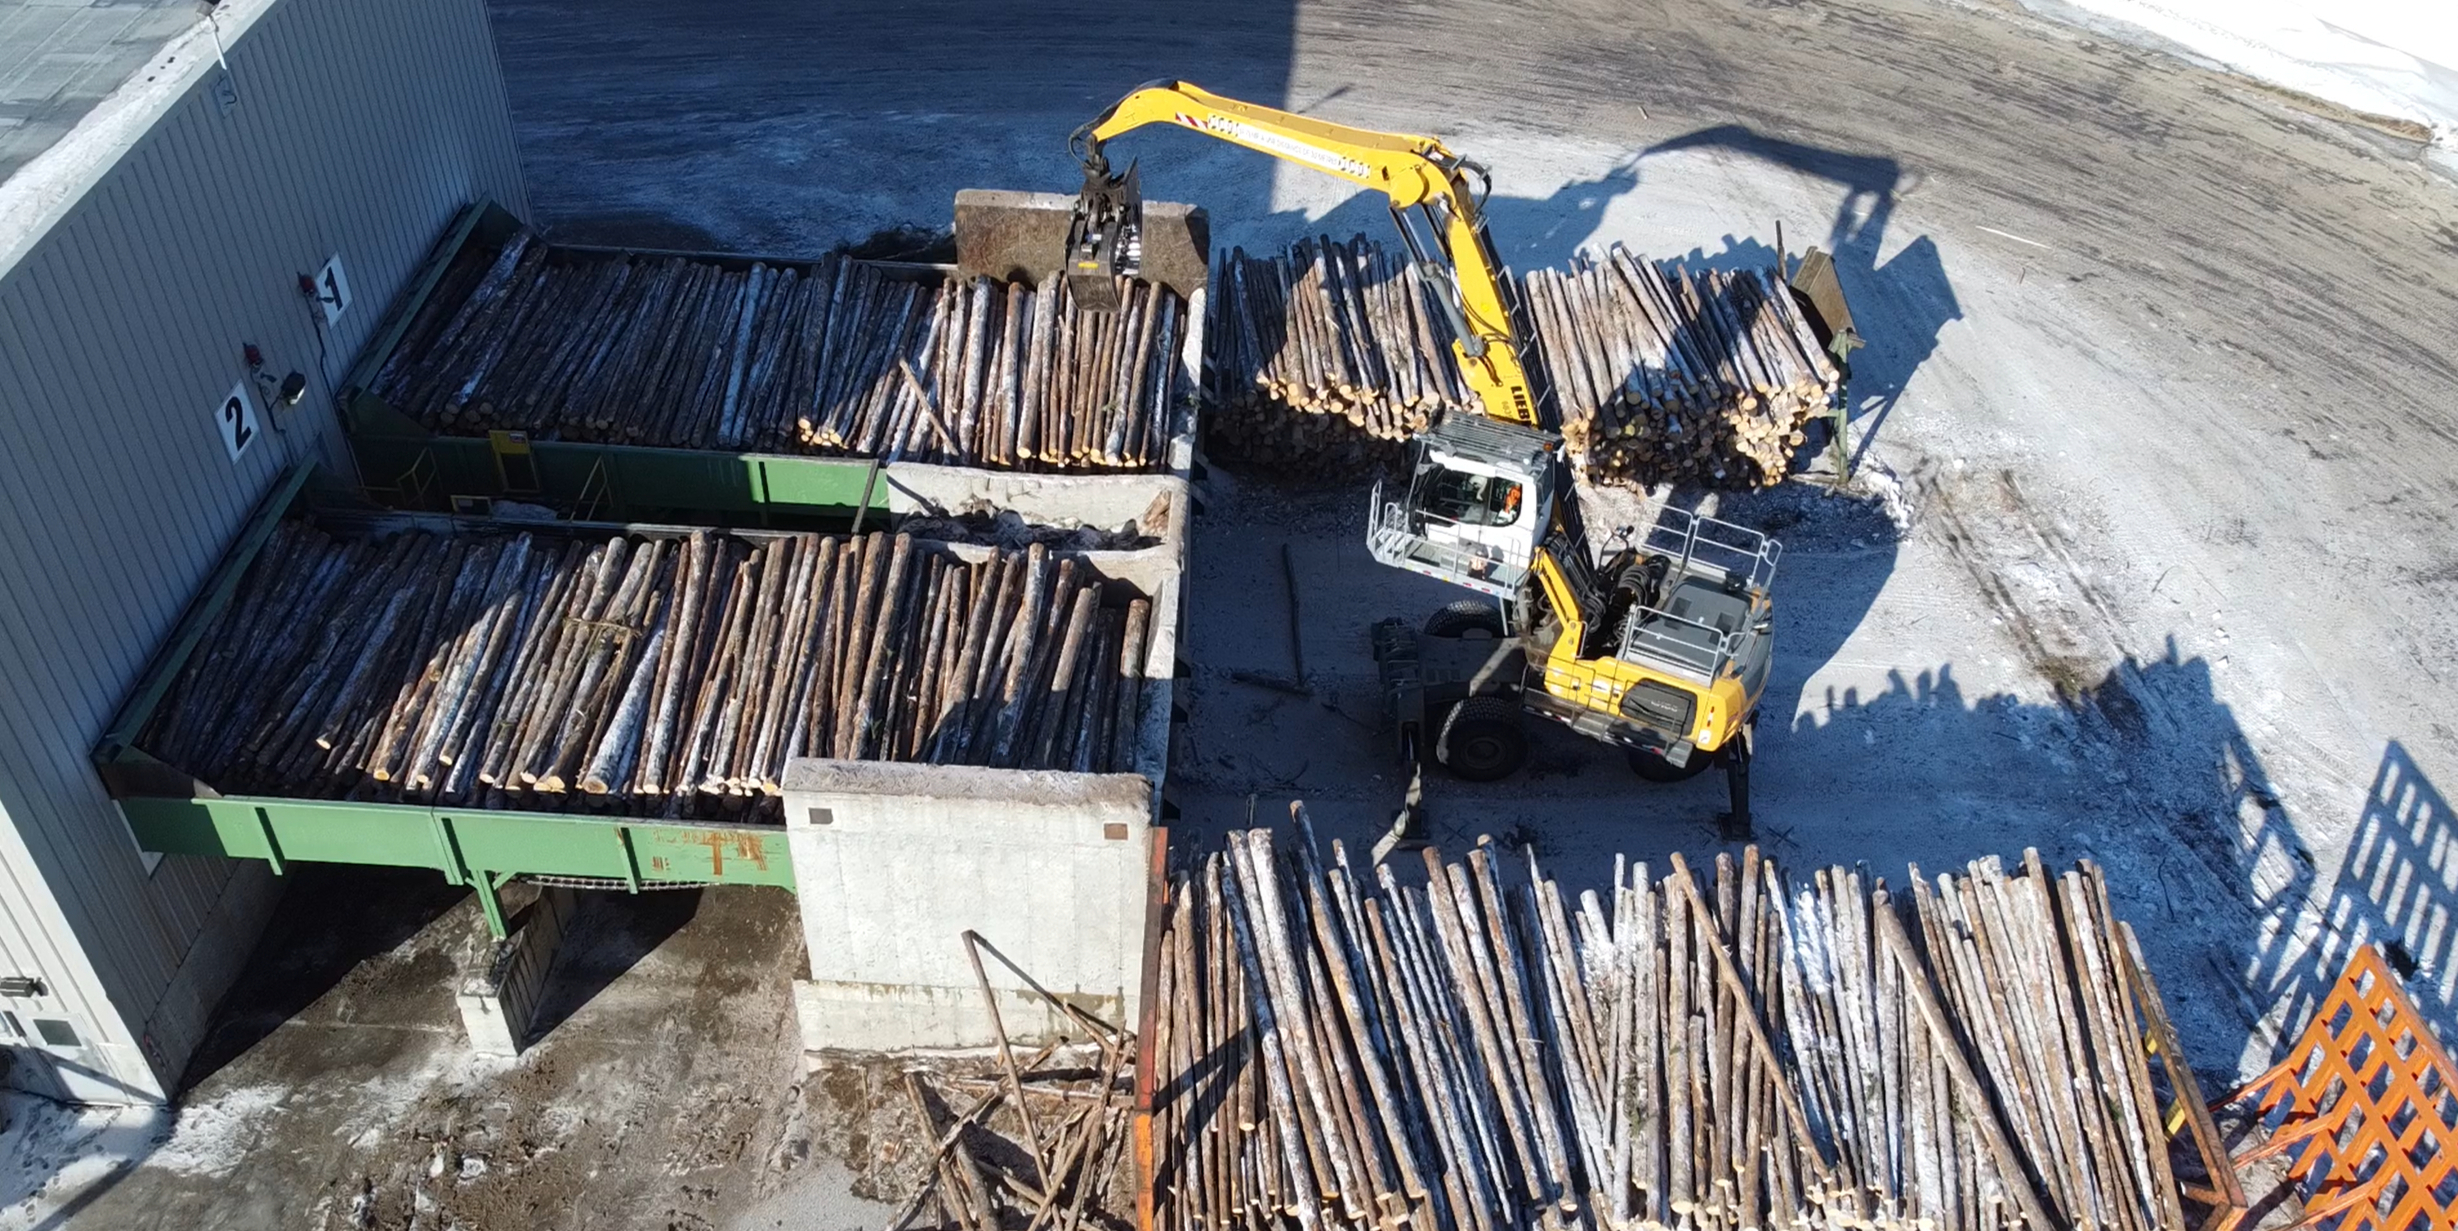
\includegraphics[width=0.85\linewidth]{mill.jpg}
\caption{A log loader clearing piles at a millyard infeed deck. The operator
repeatedly selects a grasp location and orientation on the pile, closes the
grapple over multiple logs, and transfers the load. This targeting decision is
the subject of this thesis.}
\label{fig:intro_mill}
\end{figure}

Automating the pile-clearing task is difficult for reasons that are distinct
from those studied in most robotic grasping research. The scene contains
hundreds of near-identical cylindrical logs in extensive frictional contact;
there is no notion of picking an isolated object, because the grapple executes
power grasps that capture bunches of logs at once. Every grasp disturbs the
pile through contact cascades, so the problem is inherently sequential: a good
targeting strategy must remain effective from the full, ordered stack down to
the last scattered logs. Finally, the machine perceives the pile only through
exteroceptive sensing, in this work a stereo depth camera, so decisions must be
made from partial, noisy surface observations rather than from knowledge of
every log's pose.

\section{Problem Statement}

This thesis addresses the grasp target selection problem for autonomous log
pile clearing: given a point cloud derived from a depth camera, decide where to
place the grapple and how to orient it so that the pile is cleared efficiently,
grasp after grasp. The scope is deliberately factored. The targeting decision
is learned, while motion execution remains classical: a fixed finite state
machine executes each commanded grasp cycle through inverse-kinematics control
of the crane joints. This separation concentrates the learning problem on the
part of the task that resists hand-engineering, the perception-driven decision,
and keeps the executed motions predictable and auditable, which matters on a
multi-tonne machine.

Three questions structure the work.
\begin{enumerate}
\item Can a policy learn effective sequential grasp targeting for dense piles
of hundreds of logs directly from raw, unsegmented point clouds, and what
combination of imitation and reinforcement learning gets it there?
\item How should the grasp be parameterized so that the learned policy remains
reliable under the multimodal pile geometries and the sensing artifacts of the
real machine?
\item What does it take to carry a policy trained in simulation onto a physical
crane, and how does it perform there against the deployed engineered baseline?
\end{enumerate}

The experimental platform is a full-scale log loader testbed operated with
FPInnovations, equipped with crane joint sensing, a programmable logic
controller (PLC) interface, and ZED stereo cameras. Its digital counterpart is
a GPU-parallel simulation built in Isaac Lab~\cite{mittal2025isaaclab}, tuned
to the measured properties of the physical logs and used for all training.

\section{Approach and Contributions}

The backbone of the approach is a two-stage learning pipeline. A privileged
scripted expert, which reads ground-truth log poses in simulation, generates
demonstrations of a top-of-pile targeting strategy; a PointNet-based
policy~\cite{qi2017pointnet} is trained by behavior cloning (BC) to reproduce
these decisions from raw point clouds alone; and reinforcement learning (RL)
then fine-tunes the cloned policy against the task objective, using an
asymmetric actor-critic in which the critic reads privileged state that the
deployed actor never sees~\cite{pinto2018asymmetric}. The thesis develops this
pipeline in simulation, carries it through calibration and systems integration
onto the physical crane, and closes the loop with field trials whose failure
analysis feeds back into the policy design.

The contributions are:
\begin{enumerate}
\item \emph{A simulated crane testbed for pile-scale clearing.} An Isaac Lab
environment simulating a forestry crane with a passively suspended grapple and
piles of approximately 200 logs in frictional contact, with physics parameters tuned
from field measurements, a fixed grasp-cycle state machine that isolates
targeting from execution, and a decision-level task formulation in which one
environment step is one grasp (Chapter~\ref{ch:sim_env}).
\item \emph{A simulation study of learning methods at pile scale.} A
controlled comparison of a privileged heuristic, from-scratch RL, BC, and
BC-initialized RL fine-tuning, showing that from-scratch RL fails to learn
full-trajectory clearing regardless of observation type, that BC from raw
unsegmented clouds reaches near-expert clearing, and that a frozen-encoder,
asymmetric-critic fine-tuning recipe preserves the cloned competence during RL
(Chapter~\ref{ch:sim_study}).
\item \emph{Two grasp parameterizations and their failure modes.} A regression
policy that outputs grasp coordinates and a scoring policy that classifies
which observed point to grasp, trained on identical data, with an analysis
showing that the regression policy's conditional-mean behavior produces an
absorbing grasp-over-the-gap failure on multimodal piles that the scoring
policy removes by construction (Chapter~\ref{ch:bc_policies}).
\item \emph{Calibration and deployment infrastructure for sim-to-real
transfer.} A joint-space control interface to the crane PLC with
centimeter-level task-space tracking, camera extrinsic calibration using the
grapple itself as the calibration object with a floor-constrained refinement,
fused two-camera rack localization, and a simulation environment updated to
reproduce the calibrated viewpoint and scene geometry
(Chapter~\ref{ch:sim2real}).
\item \emph{Field evidence.} A baseline campaign of the deployed geometric
heuristic on 200-log piles establishing a failure taxonomy dominated by
absorbing structure-targeting errors, and hardware trials of the learned
scoring policy demonstrating unassisted pile clearing where the baseline had
to be abandoned (Chapter~\ref{ch:bc_policies}).
\item \emph{An RL fine-tuning architecture native to the scoring
parameterization.} A categorical-over-points actor whose action distribution
is the scoring head itself, with exact admissibility masking and per-point
credit assignment, designed from the negative results of the first-generation
Gaussian fine-tuning (Chapter~\ref{ch:bcrl}).
\end{enumerate}

Parts of this work were developed in the context of an NSERC Alliance project
on autonomy for log-loading machines in Canadian mill yards, in collaboration
with FPInnovations.

\section{Thesis Organization}

Chapter~\ref{ch:background} reviews related work on forestry crane automation,
grasping in clutter, learning from demonstrations, and point cloud policy
learning. Chapter~\ref{ch:sim_env} describes the simulated crane testbed: the
machine model, the physics tuning, the grasp-cycle controller, and the task
formulation. Chapter~\ref{ch:sim_study} presents the simulation study comparing
the heuristic, RL, BC, and BC-initialized fine-tuning.
Chapter~\ref{ch:sim2real} covers the physical testbed, its control
architecture, the calibration campaign, and the alignment of the training
environment with the deployed system. Chapter~\ref{ch:bc_policies} develops
the regression and scoring behavior-cloned policies and reports the field
trials. Chapter~\ref{ch:bcrl} presents the reinforcement learning fine-tuning
of the scoring policy. Chapter~\ref{ch:conclusion} concludes and outlines
future work.
